%=========================================================================%
% KAPITOLA 2: V Ý V O J O V É - P R O S T Ř E D Í - E C L I P S E         %
\chapter{Vývojové prostředí Eclipse}                                      %
\label{chapter:eclipse_ide}
%=========================================================================%
Eclipse IDE je integrované vývojové prostředí poskytující podporu pro mnoho programovacích jazyků, jako jsou například Java, C, C++, JavaScript a PHP.  Je záložen na modulové architektuře, která umožňuje snadné rozšíření této platformy. Pro přidání nové funkcionality do vývojového prostředí stačí nainstalovat příslušný zásuvný modul (\emph{angl. plug-in}). Projekt Eclipse je udržován radou správců \emph{eclipse.org}, která vznikla z~iniciativy společností \emph{Borland}, \emph{IBM}, \emph{MERANT}, \emph{QNX Software Systems}, \emph{Rational Software}, \emph{Red Hat}, \emph{SuSE}, \emph{TogetherSoft} a \emph{Webgain}. Cílem eclipse.org je tvorba univerzálního rozšiřitelného integrovaného vývojového prostředí, které poskytuje nástroje pro integraci různých platforem a zároveň potřebné nástroje pro jejich tvorbu a rozšíření \cite{eclipse-org}.

V~následující kapitole je popsána struktura Eclipse IDE a částí, ze kterých se skládá. Dále je zde popsán systém zásuvných modulů Eclipse IDE a jejich částí.

  \section{Infrastruktura Eclipse IDE}
  \label{section:Infrastruktura_Eclipse_IDE}
  %===============================
  Eclipse IDE není monolitické vývojové prostředí, ale spíše komplexní soubor zásuvných modulů. V~základě je rozdělen do několika podsystémů, které jsou koncipovány jako jeden nebo více zásuvných modulů. Minimální množina zásuvných modulů, která je potřeba pro vývoj klientské aplikace se nazývá \emph{Eclipse RCP} (\emph{Rich Client Platform})\footnote{\url{https://wiki.eclipse.org/Rich_Client_Platform}}. V~dnešní době se však Eclipse IDE často používá i pro vývoj serverových aplikací, tato infrastruktura se potom nazývá \emph{EAF} (\emph{Eclipse Aplication Framework}). Důležitou komponentou je jádro, které načítá jednotlivé zásuvné moduly. Toto jádro je implementováno na základě specifikace \emph{OSGi Service Platform}, která definuje standard pro dynamické modulární systémy v~Javě \cite{Plugins}. Tento standard je definován mezinárodním konsorciem \emph{OSGi Alliance}\footnote{\url{https://www.osgi.org/}}. Díky implementaci rámce \emph{OSGi Equinox}\footnote{\url{http://www.eclipse.org/equinox/}} používá Eclipse IDE pro načítání jednotlivých zásuvných modulů návrhový vzor \emph{lazy-loading}, který zajišťuje načítání jen nezbytných zásuvných modulů.
  \\
  \\
  \noindent
  Zásuvné moduly se v~základu dělí podle funkce do několika skupin \cite{Plugins}:
  \begin{description}
    \item[Core:] skupina nízkoúrovňových zásuvných modulů zajišťujících základní funkce jako jsou zpracování rozšíření zásuvných modulů a zdrojových kódů.
    \item[SWT\,(Standard Widget Toolkit):] knihovna nástrojů pro manipulaci s~uživatelským rozhraním, která poskytuje API nezávislé na operačním systému.
    \item[JFace:] knihovna přidávající další funkcionalitu jako nástavbu k~SWT.
    \item[GEF:] rámec poskytující prostředí pro vývoj grafických editorů.
    \item[Workbench:] skupina zásuvných modulů poskytujících funkcionalitu specifickou přímo pro Eclipse IDE, jako je manipulace s~projekty nebo grafickými prvky (pohledy, perspektivami, atd.).
    \item[Team:] skupina zásuvných modulů poskytujících podporu pro správu verzí v~Eclipse IDE.
    \item[Help:] poskytuje dokumentaci k~jednotlivým prvkům Eclipse IDE.
    \item[JDT\,(Java Development Tools)\footnotemark:] \footnotetext{\url{http://www.eclipse.org/jdt/}} přidává podporu pro vývoj Java aplikací a navíc do Eclipse IDE přidává perspektivy, pohledy, průvodce a další nástroje pro práci s~Javou.
    \item[PDE\,(Plug-in Development Enviroment)\footnotemark:] \footnotetext{\url{http://www.eclipse.org/pde/}} skupina zásuvných modulů poskytujících různé nástroje\,(pohledy, editory, atd.) pro práci se zásuvnými moduly a jejich manifesty.
    \item[Mylyn:] poskytuje rámec pro správu úkolů a životního cyklu aplikace (Application Lifecycle Management)
  \end{description}

  \begin{figure}
    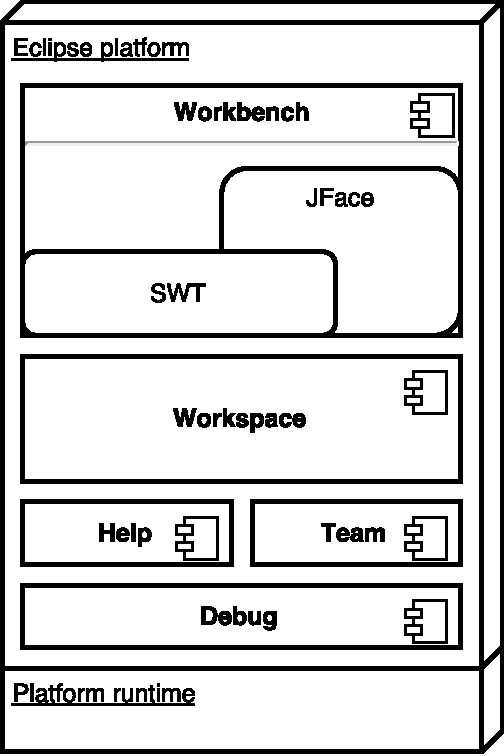
\includegraphics[width=0.5\textwidth, center]{obrazky-figures/eclipse_arch.pdf}
    \caption[Architektura platformy Eclipse.]{Architektura platformy Eclipse (inspirováno v~\cite{eclipse-platform}).}
    \label{fig:eclipse_arch}
  \end{figure}

  Na obrázku \ref{fig:eclipse_arch} jsou znázorněny základní komponenty platformy Eclipse. \emph{Workbench} představuje obálku, která umožňuje uživateli orientaci ve vývojovém prostředí. Definuje \emph{body rozšíření}\,(\emph{angl. extension points}), kde je možno k~zásuvnému modulu přidat další, rozšiřující modul. Díky těmto bodům lze přidávat například komponenty grafického rozhraní, jako jsou pohledy, editory a menu. \emph{Pracovní plocha}\,(\emph{angl. Workspace}) definuje rozhraní pro programování aplikací\,(dále zkráceně API) za účelem vytváření a správy projektů, souborů a složek. Zde jsou projekty překládány a sestavovány. Pracovní plocha navíc obsahuje další informace k~projektům, jako je například uživatelské nastavení. \emph{Help} poskytuje body rozšíření sloužící pro zobrazení nápovědy nebo dokumentace. Modul \emph{Team} definuje model pro vývoj aplikací v~týmu, s~podporou správy verzí aplikace a zdrojových kódů. Komponenta \emph{Platform Runtime} spravuje informace týkající se právě běžícího prostředí Eclipse. Například dynamicky vyhledává a spravuje informace o~zásuvných modulech a jejich bodech rozšíření. Také poskytuje informace ohledně správy procesů, argumentů příkazové řádky, adresářové struktury jednotlivých zdrojů a další \cite{Plugins}.

    \subsection{Workbench}
    %*********************
    Termín Workbench odkazuje na desktopové vývojové prostředí. Jeho cílem je integrace různých nástrojů a poskytnutí základního schématu pro tvorbu, správu a navigaci ve zdrojích pracovní plochy. Běžně se ve Workbench nachází lišta s~hlavním menu, nástrojová lišta a několik pohledů, případně editorů \cite{eclipse-workbench}. Grafické prvky vývojového prostředí jsou však pro uživatele přizpůsobitelné. Běžný vzhled Eclipse Workbench je zobrazen na obrázku \ref{fig:eclipse_workbench}.

    \begin{figure}
      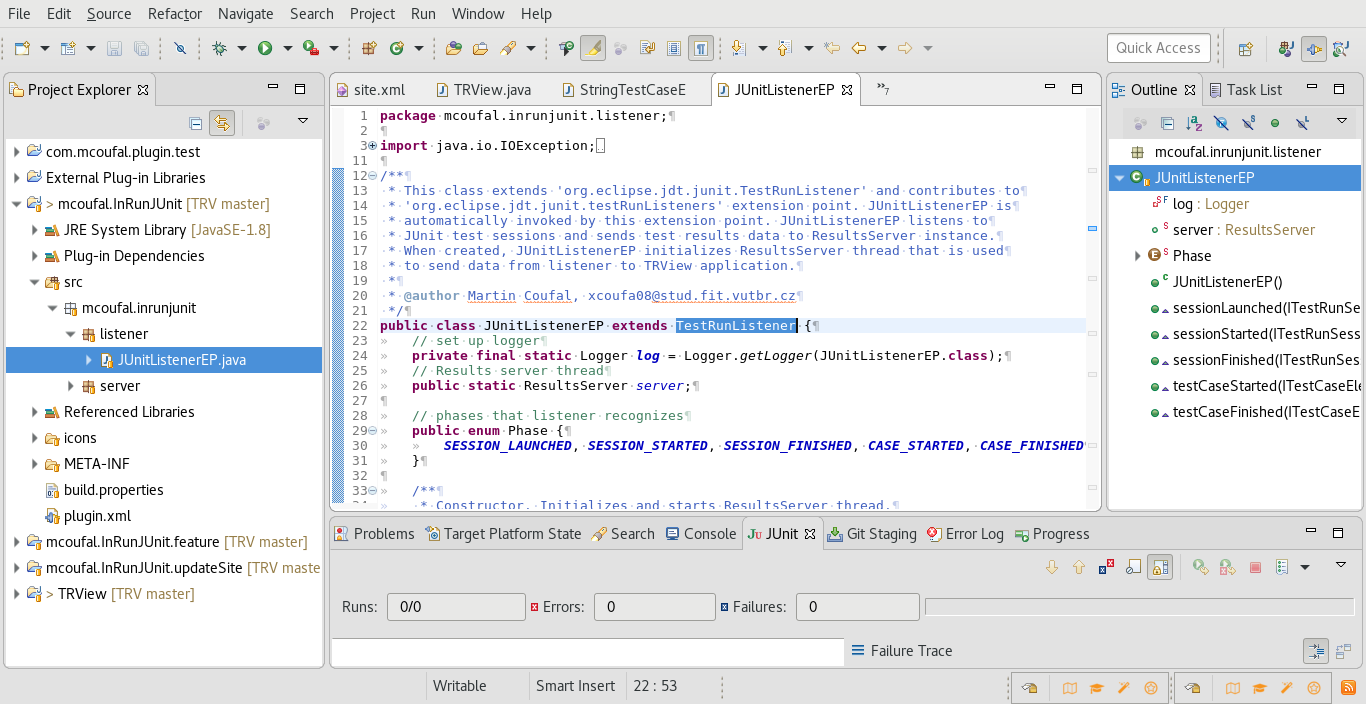
\includegraphics[width=\textwidth, keepaspectratio, center]{obrazky-figures/eclipse_workbench.png}
      \caption{Běžný vzhled Eclipse Workbench.}
      \label{fig:eclipse_workbench}
    \end{figure}

      \subsubsection{Pohledy}
      %----------------------
      Pohled je jednou ze základních komponent tvořících grafické uživatelské rozhraní Eclipse IDE. Slouží k~zobrazování informací uživateli a také k~navigaci ve vývojovém prostředí. Každý pohled může mít svá menu a své nástrojové lišty.

      Pro vytvoření nového pohledu je zapotřebí dvou kroků\,--\,vytvoření kategorie pohledu\,(pokud ho nechceme vytvořit v~některé z~již existujících kategorií) a deklarace nového pohledu. Obě dvě změny probíhají v~manifestu zásuvného modulu. Přesto, že je možné tyto změny do manifestu dopsat ručně, vývojové prostředí Eclipse nabízí praktické nástroje pro editaci manifestů zásuvných modulů. Otevření některého z~manifestů zásuvného modulu spustí editor zásuvného modulu. Nastavení rozšíření zásuvného modulu lze upravovat v~záložce \emph{Extensions}. Pro přidání kategorie pohledu i deklarace pohledu samotného je nutné nejdříve přidat správný bod rozšíření. Všechny pohledy se připojují na bod rozšíření \texttt{org.eclipse.ui.views}. K~tomuto bodu rozšíření lze přidat novou kategorii pohledu, nebo deklarovat nový pohled.

      Běžně používanou třídou implementující toto rozhraní je \texttt{org.eclipse.ui.part.ViewPart}. Zdrojový kód s~popisem chování daného pohledu se nachází ve třídě implementující rozhraní \texttt{org.eclipse.ui.IViewPart} \cite{Plugins}.

      \subsubsection{Perspektivy}
      %--------------------------
      Perspektivy slouží jako nástroj pro seskupení relevantních komponent v~aktivním okně Workbench. Komponenty se seskupují podle úkonu, který bude uživatel vykonávat a  zároveň podle programovacího jazyka, ve kterém uživatel projekt vytváří. Eclipse IDE umožňuje přidání nových perspektiv pomocí zásuvných modulů a bodů rozšíření. Pokud je to žádoucí, lze také při přidání nového zásuvného modulu některou z~již existujících perspektiv pouze upravit.

      Pro přidání nové perspektivy, podobně jako u~přidání nového pohledu, je nutno do manifestu zásuvného modulu přidat správný bod rozšíření\,--\,\texttt{org.eclipse.ui.perspectives}. Rozložení komponent v~dané perspektivě je definováno ve třídě implementující rozhraní \texttt{IPerspectiveFactory} \cite{Plugins}. Přidat nové rozšíření zásuvného modulu implementující novou nebo upravenou perspektivu lze jednoduše pomocí nástrojů v~záložce \emph{Extensions} u~editoru zásuvného modulu. Chceme-li perspektivu pouze upravit, lze při tvorbě nové perspektivy vybrat některou z~již existujících.

      \subsubsection{Editory}
      %----------------------
      Editory slouží jako hlavní nástroj pro úpravu zdrojového kódu a jiných textových souborů. Eclipse IDE nabízí mnoho editorů, které je možno nainstalovat v~rámci nějakého ze zásuvných modulů. Nejzákladnějším editorem je textový editor. Ten poskytuje pouze základní funkce pro práci s~textem a neposkytuje možnost zvýraznění syntaxe nebo její kontrolu. I~základní textový editor je však možno dále rozšířit pomocí dalších zásuvných modulů.

      Editor lze přidat pomocí rozšiřujícího bodu \texttt{org.eclipse.ui.editors}. Na ten lze připojit vlastní třídu implementující rozhraní \texttt{org.eclipse.ui.IEditorPart} \cite{Plugins}. Proces vytváření nového editoru je stejný jako v~předchozích dvou případech.

      \subsection{Standard Widget Toolkit}
      %***********************************
      SWT představuje tenkou vrstvu nad nativním ovládáním uživatelského rozhraní platformy Eclipse. Poskytuje tak rozhraní pro pohodlnější interakci s~uživatelským rozhraním, které zahrnuje většinu prvků nacházejících se v~platformě Eclipse a tak lze pomocí SWT snadno vytvářet aplikace s~grafickým uživatelským rozhraním \cite{Plugins}. Zároveň je na SWT postaven zásuvný modul \emph{SWTBot}, sloužící pro testování uživatelského rozhraní.

  \section{Architektura zásuvných modulů v~Eclipse IDE}
  %====================================================
  Každý zásuvný modul v~Eclipse IDE slouží buď jako knihovna pro dodatečné funkce jiným zásuvným modulům, nebo pro rozšíření funkcionality platformy. Chování každého zásuvného modulu je popsáno v~jeho zdrojovém kódu. Závislosti, body rozšíření a služby poskytované  zásuvným modulem jsou popsány v~manifestech zásuvného modulu\,--\,souborech \texttt{MANIFEST.MF} a \texttt{plugin.xml}. Načítání nových zásuvných modulů probíhá až když je modul přímo vyžadován\,(dle návrhového vzoru lazy-loading). Na začátku jsou načteny pouze manifesty zásuvných modulů. Ty poskytují základní informace o~zásuvném modulu a nemusí se tak načítat kompletní zásuvný modul. Díky tomuto modelu je Eclipse IDE i přes velké množství možných instalovaných zásuvných modulů kompaktnější a výrazně rychlejší při startu.

  Zásuvný modul\,(ať už v~podobě Java archivu JAR nebo v~podobě adresáře projektu) se skládá z~Javových tříd, manifestů zásuvného modulu\,(\texttt{MANIFEST.MF} a \texttt{plugin.xml}) a obrázkových souborů, které jsou typicky umístěny v~adresářích pojmenovaných \emph{icons} nebo \emph{images}. Pokud je zásuvný modul ve formě adresáře, archiv JAR je uložen v~některém z~podadresářů. Název archivu JAR a jeho umístění je v~takovém případě definováno v~souboru \texttt{MANIFEST.MF}.

    \subsection{Model zásuvných modulů}
    %********************************
    Eclipse IDE při startu prohledá všechny adresáře se zásuvnými moduly a vytvoří vlastní model obsahující každý nalezený zásuvný modul. Tento model se vytváří pomocí manifestů zásuvných modulů tak, aby Elipse nemusel načítat celé zásuvné modely a ušetřil tak čas a místo. Informace o~jednotlivých nainstalovaných zásuvných modulech jsou uloženy v~balíčcích\,(\emph{angl. bundles}). Získáváním informací přes rozhraní těchto balíčků zajistíme, aby se zásuvné moduly nenačítaly, dokud nejsou opravdu zapotřebí.

    Původně mělo Eclipse IDE vlastní mechanismus pro běh aplikace, ale to znemožnilo použití již vytvořených technologií v~jiných oblastech jako Avalon\footnote{\url{https://avalon.apache.org}} nebo JMX\footnote{\url{http://www.oracle.com/technetwork/articles/java/javamanagement-140525.html}}. Proto byl nakonec nahrazen mechanismem pro běh aplikace založeném na technologii OSGi Alliance, která poskytuje model s~detailní specifikací a podporuje dynamické chování \cite{Plugins}.

    \subsection{Vytvoření zásuvného modulu}
    %**************************************
    Pro vytvoření zásuvného modulu poskytuje platforma Eclipse zásuvný modul PDE, který poskytuje mnoho užitečných nástrojů pro tvorbu, manipulaci a distribuci zásuvných modulů. Platforma Eclipse poskytuje mnoho variant konfigurací, jaké lze stáhnout a instalovat. Zásuvný modul PDE je součástí například Eclipse SDK, Eclipse Classic a Eclipse Standard. Eclipse PDE lze také zpětně doinstalovat například pomocí \emph{Eclipse marketplace}\footnote{\url{https://marketplace.eclipse.org/content/eclipse-pde-plug-development-environment}}.

    V~PDE má každý zásuvný modul svůj vlastní projekt. Tento projekt lze vytvořit pomocí průvodce, nebo konvertovat již existující projekt na projekt se zásuvným modulem. Pro tvorbu nového projektu stačí použít průvodce \emph{New Plug-in Project}, vyplnit základní informace o~projektu, informace o~zásuvném modulu\footnote{Jednotlivé položky k~vyplnění jsou blíže popsány v~sekci \ref{section:manifesty_zasuvneho_modulu}} a dokončit průvodce \cite{Blewitt:Eclipse4}.

    \subsection{Manifesty zásuvného modulu}
    \label{section:manifesty_zasuvneho_modulu}
    %**************************************
    Manifesty zásuvného modulu jsou dva soubory\,--\,\texttt{MANIFEST.MF} a \texttt{plugin.xml}. První zmíněný obsahuje data nutná pro běh zásuvného modulu jako jsou \emph{identifikátor}, \emph{verze} a \emph{závislosti} zásuvného modulu. Druhý obsahuje data ve formátu XML popisující případná rozšíření a body rozšíření.

      \subsubsection{Soubor \texttt{MANIFEST.MF}}
      %-------------------------------------
      V~každém souboru \texttt{MANIFEST.MF} zásuvného modulu se nacházejí záznamy pro jméno, identifikátor, verzi, spouštěč a poskytovatele balíčku zásuvného modulu. Dále se zde mohou vyskytovat záznamy s~\emph{ClassPath}, exportovanými balíčky a závislostmi zásuvného modulu.

      Jméno\,(\emph{Bundle-Name}) a poskytovatel\,(\emph{Bundle-Vendor}) jsou \emph{human-readable}\footnote{\url{https://en.oxforddictionaries.com/definition/us/human-readable}} řetězce, které nemusí být unikátní a lze je ukládat do zvláštního souboru \texttt{plugin.properties} za účelem internacionalizace.

      Identifikátor\,(\emph{Bundle-SymbolicName}) slouží k~jednoznačné identifikaci daného balíčku. Většinou se jako identifikátor balíčku používá Javová konvence pro pojmenování balíčků: \texttt{com.<název společnosti>.<komponenta>[.<část komponenty>]}, kde část dané komponenty\,(například '\texttt{ui}' nebo '\texttt{core}') se uvádí v~případě větších komponent, kde jsou jednotlivé balíčky rozděleny. U~tohoto identifikátoru bývá ještě uvedena direktiva OSGi \texttt{singleton}, která udává zda může být v~platformě instalováno více verzí daného zásuvného modulu současně \cite{Blewitt:Eclipse4}.

      Verze\,(\emph{Bundle-Version}) slouží k~jednoznačné identifikaci verze daného balíčku. V~případě shody identifikátorů je vždy vybrán balíček s~novějším číslem verze. Toto číslo se skládá ze 3 číslic oddělených tečkami a v~případě potřeby i alfanumerického řetězce použitelného pro užší specifikaci\,(například '\texttt{1.2.3.beta}'). První číslo označuje majoritní verzi produktu, druhé minoritní verzi produktu a třetí slouží k~označení úrovně služeb\footnote{více k~číslování balíčků lze nalézt na \url{https://wiki.eclipse.org/Version_Numbering}}.

      Spouštěč\,(\emph{Bundle-Activator}) je volitelná část manifestu která umožňuje specifikovat třídu implementující rozhraní \texttt{BundleActivator} a poskytuje tak metody \texttt{start()} a \texttt{stop()}, které jsou přínosné pro správu životního cyklu balíčku.

      \emph{Bundle-ClassPath} je záznam využitý pro seznam balíčků a knihoven, které mají být do zásuvného modulu přidány. Modul tak může být instalován sám o~sobě bez nutnosti stahování dalších balíčků nebo knihoven\footnote{Takto přidané balíčky však výrazně zvětšují velikost výsledného zásuvného modulu.}.

      Záznam s~exportovanými balíčky\,(\emph{Export-Package}) je podmnožina z~Bundle-ClassPath obsahující balíčky, které mají být viditelné pro ostatní balíčky zásuvných modulů.

      Eclipse IDE vytváří pro každý načtený zásuvný modul novou instanci, která slouží k~vyhledávání a načítání zásuvných modulů a používá \emph{záznam závislostí} v~manifestu k~určení viditelnosti ostatních zásuvných modulů. Záznam závislostí\,(\emph{Require-Bundle}) je seznam zásuvných modulů, které jsou pro daný zásuvný modul viditelné z~hlediska vykonávání programu \cite{Plugins}.

      \subsubsection{Soubor \texttt{plugin.xml}}
      %------------------------------------
      V~tomto manifestu zásuvného modulu mohou být uvedeny body rozšíření, na které je možno připojit nový zásuvný modul rozšiřující stávající funkcionalitu. Toto odloučení od rozšiřujících zásuvných modulů umožňuje existenci základního zásuvného modulu bez znalosti jakýchkoliv informací o~ostatních zásuvných modulech. To zajišťuje snazší spolupráci při implementaci a znovupoužitelnost již implementovaných částí \cite{Plugins}. Bod rozšíření obvykle definuje identifikátor, jméno a schéma\,(viz obrázek \ref{code:extension_point_declaration}). Schéma určuje, co musí rozšiřující zásuvný modul splnit pro správné rozšíření tohoto zásuvného modulu. Deklarace bodu rozšíření se vkládá do bloku s~označením \texttt{<plugin>}. 

      \lstset{language=xml}
      \begin{figure}
	\begin{lstlisting}[frame=single]
<extension-point id="org.example.extensionpoints.point"
  name="Point"
  schema="schemas/scheme.exsd" />
	\end{lstlisting}
	\caption{Příklad zdrojového kódu s~definicí bodu rozšíření.}
	\label{code:extension_point_declaration}
      \end{figure}

      Dále je zde možno definovat, který zásuvný modul chceme stávajícím modulem rozšířit\,--\,k tomu slouží rozšíření zásuvného modulu\,(viz obrázek \ref{code:extension_declaration}). Obsah bloku \texttt{<extension point>} je dán bodem rozšíření na který se připojujeme. V~případě obrázku \ref{code:extension_declaration} jde o~připojení na bod rozšíření \texttt{org.eclipse.ui.views}, který umožňuje přidání vlastního pohledu. K~tomu je třeba specifikovat kategorii\,(v případě že vytváříme novou) a zároveň jednotlivé parametry implementovaného pohledu.

      \begin{figure}
	\begin{lstlisting}[frame=single]
<extension
  point="org.eclipse.ui.views">
  <category
    id="com.example.myview"
    name="Sample Category">
  </category>
  <view
    category="com.example.myview"
    class="com.example.myview.views.SampleView"
    icon="icons/sample.gif"
    id="com.example.myview.views.SampleView"
    name="Sample View">
  </view>
</extension>
	\end{lstlisting}
	\caption{Příklad zdrojového kódu s~připojením na bod rozšíření \texttt{org.eclipse.ui.views}.}
	\label{code:extension_declaration}
      \end{figure}